\documentclass[1p]{elsarticle_modified}
%\bibliographystyle{elsarticle-num}

%\usepackage[colorlinks]{hyperref}
%\usepackage{abbrmath_seonhwa} %\Abb, \Ascr, \Acal ,\Abf, \Afrak
\usepackage{amsfonts}
\usepackage{amssymb}
\usepackage{amsmath}
\usepackage{amsthm}
\usepackage{scalefnt}
\usepackage{amsbsy}
\usepackage{kotex}
\usepackage{caption}
\usepackage{subfig}
\usepackage{color}
\usepackage{graphicx}
\usepackage{xcolor} %% white, black, red, green, blue, cyan, magenta, yellow
\usepackage{float}
\usepackage{setspace}
\usepackage{hyperref}

\usepackage{tikz}
\usetikzlibrary{arrows}

\usepackage{multirow}
\usepackage{array} % fixed length table
\usepackage{hhline}

%%%%%%%%%%%%%%%%%%%%%
\makeatletter
\renewcommand*\env@matrix[1][\arraystretch]{%
	\edef\arraystretch{#1}%
	\hskip -\arraycolsep
	\let\@ifnextchar\new@ifnextchar
	\array{*\c@MaxMatrixCols c}}
\makeatother %https://tex.stackexchange.com/questions/14071/how-can-i-increase-the-line-spacing-in-a-matrix
%%%%%%%%%%%%%%%

\usepackage[normalem]{ulem}

\newcommand{\msout}[1]{\ifmmode\text{\sout{\ensuremath{#1}}}\else\sout{#1}\fi}
%SOURCE: \msout is \stkout macro in https://tex.stackexchange.com/questions/20609/strikeout-in-math-mode

\newcommand{\cancel}[1]{
	\ifmmode
	{\color{red}\msout{#1}}
	\else
	{\color{red}\sout{#1}}
	\fi
}

\newcommand{\add}[1]{
	{\color{blue}\uwave{#1}}
}

\newcommand{\replace}[2]{
	\ifmmode
	{\color{red}\msout{#1}}{\color{blue}\uwave{#2}}
	\else
	{\color{red}\sout{#1}}{\color{blue}\uwave{#2}}
	\fi
}

\newcommand{\Sol}{\mathcal{S}} %segment
\newcommand{\D}{D} %diagram
\newcommand{\A}{\mathcal{A}} %arc


%%%%%%%%%%%%%%%%%%%%%%%%%%%%%5 test

\def\sl{\operatorname{\textup{SL}}(2,\Cbb)}
\def\psl{\operatorname{\textup{PSL}}(2,\Cbb)}
\def\quan{\mkern 1mu \triangleright \mkern 1mu}

\theoremstyle{definition}
\newtheorem{thm}{Theorem}[section]
\newtheorem{prop}[thm]{Proposition}
\newtheorem{lem}[thm]{Lemma}
\newtheorem{ques}[thm]{Question}
\newtheorem{cor}[thm]{Corollary}
\newtheorem{defn}[thm]{Definition}
\newtheorem{exam}[thm]{Example}
\newtheorem{rmk}[thm]{Remark}
\newtheorem{alg}[thm]{Algorithm}

\newcommand{\I}{\sqrt{-1}}
\begin{document}

%\begin{frontmatter}
%
%\title{Boundary parabolic representations of knots up to 8 crossings}
%
%%% Group authors per affiliation:
%\author{Yunhi Cho} 
%\address{Department of Mathematics, University of Seoul, Seoul, Korea}
%\ead{yhcho@uos.ac.kr}
%
%
%\author{Seonhwa Kim} %\fnref{s_kim}}
%\address{Center for Geometry and Physics, Institute for Basic Science, Pohang, 37673, Korea}
%\ead{ryeona17@ibs.re.kr}
%
%\author{Hyuk Kim}
%\address{Department of Mathematical Sciences, Seoul National University, Seoul 08826, Korea}
%\ead{hyukkim@snu.ac.kr}
%
%\author{Seokbeom Yoon}
%\address{Department of Mathematical Sciences, Seoul National University, Seoul, 08826,  Korea}
%\ead{sbyoon15@snu.ac.kr}
%
%\begin{abstract}
%We find all boundary parabolic representation of knots up to 8 crossings.
%
%\end{abstract}
%\begin{keyword}
%    \MSC[2010] 57M25 
%\end{keyword}
%
%\end{frontmatter}

%\linenumbers
%\tableofcontents
%
\newcommand\colored[1]{\textcolor{white}{\rule[-0.35ex]{0.8em}{1.4ex}}\kern-0.8em\color{red} #1}%
%\newcommand\colored[1]{\textcolor{white}{ #1}\kern-2.17ex	\textcolor{white}{ #1}\kern-1.81ex	\textcolor{white}{ #1}\kern-2.15ex\color{red}#1	}

{\Large $\underline{11a_{302}~(K11a_{302})}$}

\setlength{\tabcolsep}{10pt}
\renewcommand{\arraystretch}{1.6}
\vspace{1cm}\begin{tabular}{m{100pt}>{\centering\arraybackslash}m{274pt}}
\multirow{5}{120pt}{
	\centering
	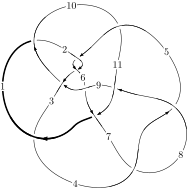
\includegraphics[width=112pt]{../../../GIT/diagram.site/Diagrams/png/551_11a_302.png}\\
\ \ \ A knot diagram\footnotemark}&
\allowdisplaybreaks
\textbf{Linearized knot diagam} \\
\cline{2-2}
 &
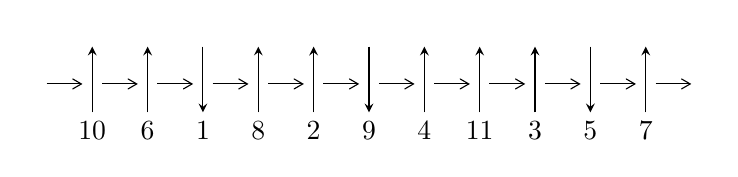
\begin{tikzpicture}[x=20pt, y=17pt]
	% nodes
	\node (C0) at (0, 0) {};
	\node (C1) at (1, 0) {};
	\node (C1U) at (1, +1) {};
	\node (C1D) at (1, -1) {10};

	\node (C2) at (2, 0) {};
	\node (C2U) at (2, +1) {};
	\node (C2D) at (2, -1) {6};

	\node (C3) at (3, 0) {};
	\node (C3U) at (3, +1) {};
	\node (C3D) at (3, -1) {1};

	\node (C4) at (4, 0) {};
	\node (C4U) at (4, +1) {};
	\node (C4D) at (4, -1) {8};

	\node (C5) at (5, 0) {};
	\node (C5U) at (5, +1) {};
	\node (C5D) at (5, -1) {2};

	\node (C6) at (6, 0) {};
	\node (C6U) at (6, +1) {};
	\node (C6D) at (6, -1) {9};

	\node (C7) at (7, 0) {};
	\node (C7U) at (7, +1) {};
	\node (C7D) at (7, -1) {4};

	\node (C8) at (8, 0) {};
	\node (C8U) at (8, +1) {};
	\node (C8D) at (8, -1) {11};

	\node (C9) at (9, 0) {};
	\node (C9U) at (9, +1) {};
	\node (C9D) at (9, -1) {3};

	\node (C10) at (10, 0) {};
	\node (C10U) at (10, +1) {};
	\node (C10D) at (10, -1) {5};

	\node (C11) at (11, 0) {};
	\node (C11U) at (11, +1) {};
	\node (C11D) at (11, -1) {7};
	\node (C12) at (12, 0) {};

	% arrows
	\draw[->,>={angle 60}]
	(C0) edge (C1) (C1) edge (C2) (C2) edge (C3) (C3) edge (C4) (C4) edge (C5) (C5) edge (C6) (C6) edge (C7) (C7) edge (C8) (C8) edge (C9) (C9) edge (C10) (C10) edge (C11) (C11) edge (C12) ;	\draw[->,>=stealth]
	(C1D) edge (C1U) (C2D) edge (C2U) (C3U) edge (C3D) (C4D) edge (C4U) (C5D) edge (C5U) (C6U) edge (C6D) (C7D) edge (C7U) (C8D) edge (C8U) (C9D) edge (C9U) (C10U) edge (C10D) (C11D) edge (C11U) ;
	\end{tikzpicture} \\
\hhline{~~} \\& 
\textbf{Solving Sequence} \\ \cline{2-2} 
 &
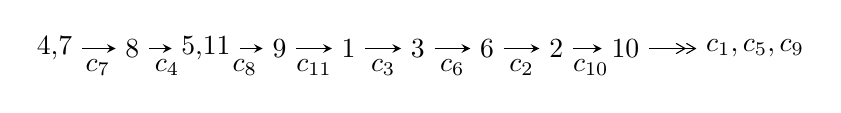
\begin{tikzpicture}[x=25pt, y=7pt]
	% node
	\node (A0) at (-1/8, 0) {4,7};
	\node (A1) at (1, 0) {8};
	\node (A2) at (33/16, 0) {5,11};
	\node (A3) at (25/8, 0) {9};
	\node (A4) at (33/8, 0) {1};
	\node (A5) at (41/8, 0) {3};
	\node (A6) at (49/8, 0) {6};
	\node (A7) at (57/8, 0) {2};
	\node (A8) at (65/8, 0) {10};
	\node (C1) at (1/2, -1) {$c_{7}$};
	\node (C2) at (3/2, -1) {$c_{4}$};
	\node (C3) at (21/8, -1) {$c_{8}$};
	\node (C4) at (29/8, -1) {$c_{11}$};
	\node (C5) at (37/8, -1) {$c_{3}$};
	\node (C6) at (45/8, -1) {$c_{6}$};
	\node (C7) at (53/8, -1) {$c_{2}$};
	\node (C8) at (61/8, -1) {$c_{10}$};
	\node (A9) at (10, 0) {$c_{1},c_{5},c_{9}$};

	% edge
	\draw[->,>=stealth]	
	(A0) edge (A1) (A1) edge (A2) (A2) edge (A3) (A3) edge (A4) (A4) edge (A5) (A5) edge (A6) (A6) edge (A7) (A7) edge (A8) ;
	\draw[->>,>={angle 60}]	
	(A8) edge (A9);
\end{tikzpicture} \\ 

\end{tabular} \\

\footnotetext{
The image of knot diagram is generated by the software ``\textbf{Draw programme}" developed by Andrew Bartholomew(\url{http://www.layer8.co.uk/maths/draw/index.htm\#Running-draw}), where we modified some parts for our purpose(\url{https://github.com/CATsTAILs/LinksPainter}).
}\phantom \\ \newline 
\centering \textbf{Ideals for irreducible components\footnotemark of $X_{\text{par}}$} 
 
\begin{align*}
I^u_{1}&=\langle 
86810 u^{20}-51179 u^{19}+\cdots+203617 b-498356,\\
\phantom{I^u_{1}}&\phantom{= \langle  }548161 u^{20}-27309 u^{19}+\cdots+203617 a+1419959,\;u^{21}-7 u^{19}+\cdots+5 u+1\rangle \\
I^u_{2}&=\langle 
1.93742\times10^{205} u^{83}-1.36676\times10^{204} u^{82}+\cdots+2.85391\times10^{204} b+1.87510\times10^{205},\\
\phantom{I^u_{2}}&\phantom{= \langle  }-8.01634\times10^{204} u^{83}-1.47295\times10^{204} u^{82}+\cdots+2.85391\times10^{204} a-2.38032\times10^{205},\\
\phantom{I^u_{2}}&\phantom{= \langle  }u^{84}+u^{83}+\cdots+13 u+1\rangle \\
I^u_{3}&=\langle 
330474083 u^{21}+170598791 u^{20}+\cdots+332950103 b-35950927,\\
\phantom{I^u_{3}}&\phantom{= \langle  }-211438488 u^{21}+97373739 u^{20}+\cdots+332950103 a+43876857,\;u^{22}-6 u^{20}+\cdots- u+1\rangle \\
I^u_{4}&=\langle 
b+u,\;u^2+a,\;u^3- u+1\rangle \\
\\
\end{align*}
\raggedright * 4 irreducible components of $\dim_{\mathbb{C}}=0$, with total 130 representations.\\
\footnotetext{All coefficients of polynomials are rational numbers. But the coefficients are sometimes approximated in decimal forms when there is not enough margin.}
\newpage
\renewcommand{\arraystretch}{1}
\centering \section*{I. $I^u_{1}= \langle 86810 u^{20}-51179 u^{19}+\cdots+203617 b-498356,\;5.48\times10^{5} u^{20}-2.73\times10^{4} u^{19}+\cdots+2.04\times10^{5} a+1.42\times10^{6},\;u^{21}-7 u^{19}+\cdots+5 u+1 \rangle$}
\flushleft \textbf{(i) Arc colorings}\\
\begin{tabular}{m{7pt} m{180pt} m{7pt} m{180pt} }
\flushright $a_{4}=$&$\begin{pmatrix}0\\u\end{pmatrix}$ \\
\flushright $a_{7}=$&$\begin{pmatrix}1\\0\end{pmatrix}$ \\
\flushright $a_{8}=$&$\begin{pmatrix}1\\- u^2\end{pmatrix}$ \\
\flushright $a_{5}=$&$\begin{pmatrix}u\\- u^3+u\end{pmatrix}$ \\
\flushright $a_{11}=$&$\begin{pmatrix}-2.69212 u^{20}+0.134119 u^{19}+\cdots-28.2075 u-6.97368\\-0.426340 u^{20}+0.251349 u^{19}+\cdots+7.71376 u+2.44752\end{pmatrix}$ \\
\flushright $a_{9}=$&$\begin{pmatrix}-1.85734 u^{20}+0.844581 u^{19}+\cdots-20.6981 u-4.31433\\0.385469 u^{20}+0.103538 u^{19}+\cdots+11.0661 u+3.11846\end{pmatrix}$ \\
\flushright $a_{1}=$&$\begin{pmatrix}-3.11846 u^{20}+0.385469 u^{19}+\cdots-20.4938 u-4.52616\\-0.426340 u^{20}+0.251349 u^{19}+\cdots+7.71376 u+2.44752\end{pmatrix}$ \\
\flushright $a_{3}=$&$\begin{pmatrix}-0.482258 u^{20}-0.0237357 u^{19}+\cdots-5.29877 u-0.756499\\-0.287854 u^{20}+0.284623 u^{19}+\cdots-5.89970 u-1.78023\end{pmatrix}$ \\
\flushright $a_{6}=$&$\begin{pmatrix}0.979437 u^{20}+0.0931160 u^{19}+\cdots-4.09981 u-0.575374\\0.0237357 u^{20}+0.194404 u^{19}+\cdots-1.65479 u-0.482258\end{pmatrix}$ \\
\flushright $a_{2}=$&$\begin{pmatrix}-0.575374 u^{20}-0.979437 u^{19}+\cdots+0.173792 u+0.222938\\-0.482258 u^{20}-0.0237357 u^{19}+\cdots-5.29877 u-1.75650\end{pmatrix}$ \\
\flushright $a_{10}=$&$\begin{pmatrix}-3.91939 u^{20}+0.521779 u^{19}+\cdots-30.2187 u-6.71970\\-1.01138 u^{20}+0.674192 u^{19}+\cdots+6.41358 u+3.08915\end{pmatrix}$\\ \flushright $a_{10}=$&$\begin{pmatrix}-3.91939 u^{20}+0.521779 u^{19}+\cdots-30.2187 u-6.71970\\-1.01138 u^{20}+0.674192 u^{19}+\cdots+6.41358 u+3.08915\end{pmatrix}$\\&\end{tabular}
\flushleft \textbf{(ii) Obstruction class $= -1$}\\~\\
\flushleft \textbf{(iii) Cusp Shapes $= \frac{338440}{203617} u^{20}+\frac{515137}{203617} u^{19}+\cdots+\frac{12952739}{203617} u+\frac{6217185}{203617}$}\\~\\
\newpage\renewcommand{\arraystretch}{1}
\flushleft \textbf{(iv) u-Polynomials at the component}\newline \\
\begin{tabular}{m{50pt}|m{274pt}}
Crossings & \hspace{64pt}u-Polynomials at each crossing \\
\hline $$\begin{aligned}c_{1},c_{8}\end{aligned}$$&$\begin{aligned}
&u^{21}-2 u^{20}+\cdots+u+1
\end{aligned}$\\
\hline $$\begin{aligned}c_{2},c_{4},c_{5}\\c_{7}\end{aligned}$$&$\begin{aligned}
&u^{21}-7 u^{19}+\cdots+5 u-1
\end{aligned}$\\
\hline $$\begin{aligned}c_{3},c_{6}\end{aligned}$$&$\begin{aligned}
&u^{21}- u^{20}+\cdots+8 u-4
\end{aligned}$\\
\hline $$\begin{aligned}c_{9},c_{11}\end{aligned}$$&$\begin{aligned}
&u^{21}-7 u^{19}+\cdots-3 u-1
\end{aligned}$\\
\hline $$\begin{aligned}c_{10}\end{aligned}$$&$\begin{aligned}
&u^{21}-7 u^{20}+\cdots+256 u-64
\end{aligned}$\\
\hline
\end{tabular}\\~\\
\newpage\renewcommand{\arraystretch}{1}
\flushleft \textbf{(v) Riley Polynomials at the component}\newline \\
\begin{tabular}{m{50pt}|m{274pt}}
Crossings & \hspace{64pt}Riley Polynomials at each crossing \\
\hline $$\begin{aligned}c_{1},c_{8}\end{aligned}$$&$\begin{aligned}
&y^{21}+32 y^{19}+\cdots+25 y-1
\end{aligned}$\\
\hline $$\begin{aligned}c_{2},c_{4},c_{5}\\c_{7}\end{aligned}$$&$\begin{aligned}
&y^{21}-14 y^{20}+\cdots+7 y-1
\end{aligned}$\\
\hline $$\begin{aligned}c_{3},c_{6}\end{aligned}$$&$\begin{aligned}
&y^{21}+17 y^{20}+\cdots-192 y-16
\end{aligned}$\\
\hline $$\begin{aligned}c_{9},c_{11}\end{aligned}$$&$\begin{aligned}
&y^{21}-14 y^{20}+\cdots+7 y-1
\end{aligned}$\\
\hline $$\begin{aligned}c_{10}\end{aligned}$$&$\begin{aligned}
&y^{21}+9 y^{20}+\cdots-32768 y-4096
\end{aligned}$\\
\hline
\end{tabular}\\~\\
\newpage\flushleft \textbf{(vi) Complex Volumes and Cusp Shapes}
$$\begin{array}{c|c|c}  
\text{Solutions to }I^u_{1}& \I (\text{vol} + \sqrt{-1}CS) & \text{Cusp shape}\\
 \hline 
\begin{aligned}
u &= \phantom{-}0.928185 + 0.189936 I \\
a &= \phantom{-}0.674396 - 0.216214 I \\
b &= -0.735536 - 1.073720 I\end{aligned}
 & \phantom{-}3.43423 + 3.77228 I & \phantom{-}11.55133 - 4.69984 I \\ \hline\begin{aligned}
u &= \phantom{-}0.928185 - 0.189936 I \\
a &= \phantom{-}0.674396 + 0.216214 I \\
b &= -0.735536 + 1.073720 I\end{aligned}
 & \phantom{-}3.43423 - 3.77228 I & \phantom{-}11.55133 + 4.69984 I \\ \hline\begin{aligned}
u &= -0.827440 + 0.723293 I \\
a &= \phantom{-}0.126743 - 0.809716 I \\
b &= \phantom{-}0.567919 - 0.288839 I\end{aligned}
 & \phantom{-}2.18487 - 3.00976 I & \phantom{-}10.87376 - 0.69402 I \\ \hline\begin{aligned}
u &= -0.827440 - 0.723293 I \\
a &= \phantom{-}0.126743 + 0.809716 I \\
b &= \phantom{-}0.567919 + 0.288839 I\end{aligned}
 & \phantom{-}2.18487 + 3.00976 I & \phantom{-}10.87376 + 0.69402 I \\ \hline\begin{aligned}
u &= -0.067511 + 1.157490 I \\
a &= \phantom{-}0.0502069 - 0.0817577 I \\
b &= \phantom{-}0.997381 - 0.629444 I\end{aligned}
 & \phantom{-}1.79260 - 6.58426 I & \phantom{-}8.00865 + 7.58329 I \\ \hline\begin{aligned}
u &= -0.067511 - 1.157490 I \\
a &= \phantom{-}0.0502069 + 0.0817577 I \\
b &= \phantom{-}0.997381 + 0.629444 I\end{aligned}
 & \phantom{-}1.79260 + 6.58426 I & \phantom{-}8.00865 - 7.58329 I \\ \hline\begin{aligned}
u &= \phantom{-}1.111710 + 0.428960 I \\
a &= -1.95911 + 0.31173 I \\
b &= \phantom{-}1.78476 + 0.65605 I\end{aligned}
 & \phantom{-}4.95885 + 9.25397 I & \phantom{-}8.29327 - 10.96531 I \\ \hline\begin{aligned}
u &= \phantom{-}1.111710 - 0.428960 I \\
a &= -1.95911 - 0.31173 I \\
b &= \phantom{-}1.78476 - 0.65605 I\end{aligned}
 & \phantom{-}4.95885 - 9.25397 I & \phantom{-}8.29327 + 10.96531 I \\ \hline\begin{aligned}
u &= -1.205890 + 0.106741 I \\
a &= -1.92936 + 0.40120 I \\
b &= \phantom{-}1.207310 + 0.326297 I\end{aligned}
 & \phantom{-}8.49324 - 2.76851 I & \phantom{-}15.4777 + 0.9885 I \\ \hline\begin{aligned}
u &= -1.205890 - 0.106741 I \\
a &= -1.92936 - 0.40120 I \\
b &= \phantom{-}1.207310 - 0.326297 I\end{aligned}
 & \phantom{-}8.49324 + 2.76851 I & \phantom{-}15.4777 - 0.9885 I\\
 \hline 
 \end{array}$$\newpage$$\begin{array}{c|c|c}  
\text{Solutions to }I^u_{1}& \I (\text{vol} + \sqrt{-1}CS) & \text{Cusp shape}\\
 \hline 
\begin{aligned}
u &= -0.789234\phantom{ +0.000000I} \\
a &= \phantom{-}1.20750\phantom{ +0.000000I} \\
b &= -0.556308\phantom{ +0.000000I}\end{aligned}
 & \phantom{-}1.38786\phantom{ +0.000000I} & \phantom{-}6.70340\phantom{ +0.000000I} \\ \hline\begin{aligned}
u &= \phantom{-}1.188640 + 0.329356 I \\
a &= -1.011510 - 0.120494 I \\
b &= \phantom{-}0.284184 - 0.245258 I\end{aligned}
 & \phantom{-}5.15265 + 4.73162 I & \phantom{-}8.09798 - 4.44428 I \\ \hline\begin{aligned}
u &= \phantom{-}1.188640 - 0.329356 I \\
a &= -1.011510 + 0.120494 I \\
b &= \phantom{-}0.284184 + 0.245258 I\end{aligned}
 & \phantom{-}5.15265 - 4.73162 I & \phantom{-}8.09798 + 4.44428 I \\ \hline\begin{aligned}
u &= -0.372563 + 0.410285 I \\
a &= -0.39105 + 1.43567 I \\
b &= -0.909633 - 0.829475 I\end{aligned}
 & \phantom{-}0.48724 + 1.81194 I & \phantom{-}3.30153 - 2.05952 I \\ \hline\begin{aligned}
u &= -0.372563 - 0.410285 I \\
a &= -0.39105 - 1.43567 I \\
b &= -0.909633 + 0.829475 I\end{aligned}
 & \phantom{-}0.48724 - 1.81194 I & \phantom{-}3.30153 + 2.05952 I \\ \hline\begin{aligned}
u &= \phantom{-}1.36146 + 0.57065 I \\
a &= \phantom{-}0.843025 - 0.608835 I \\
b &= -1.304890 + 0.034538 I\end{aligned}
 & \phantom{-}10.21620 + 5.64989 I & \phantom{-}15.0241 - 3.8611 I \\ \hline\begin{aligned}
u &= \phantom{-}1.36146 - 0.57065 I \\
a &= \phantom{-}0.843025 + 0.608835 I \\
b &= -1.304890 - 0.034538 I\end{aligned}
 & \phantom{-}10.21620 - 5.64989 I & \phantom{-}15.0241 + 3.8611 I \\ \hline\begin{aligned}
u &= -1.41669 + 0.52365 I \\
a &= \phantom{-}1.55271 + 0.10596 I \\
b &= -1.38942 + 1.03688 I\end{aligned}
 & \phantom{-}11.2036 - 18.3943 I & \phantom{-}11.0076 + 9.0976 I \\ \hline\begin{aligned}
u &= -1.41669 - 0.52365 I \\
a &= \phantom{-}1.55271 - 0.10596 I \\
b &= -1.38942 - 1.03688 I\end{aligned}
 & \phantom{-}11.2036 + 18.3943 I & \phantom{-}11.0076 - 9.0976 I \\ \hline\begin{aligned}
u &= -0.305278 + 0.294373 I \\
a &= \phantom{-}0.94021 - 1.42121 I \\
b &= -0.223914 + 0.503703 I\end{aligned}
 & \phantom{-}0.730644 - 1.059890 I & \phantom{-}8.01231 + 6.34216 I\\
 \hline 
 \end{array}$$\newpage$$\begin{array}{c|c|c}  
\text{Solutions to }I^u_{1}& \I (\text{vol} + \sqrt{-1}CS) & \text{Cusp shape}\\
 \hline 
\begin{aligned}
u &= -0.305278 - 0.294373 I \\
a &= \phantom{-}0.94021 + 1.42121 I \\
b &= -0.223914 - 0.503703 I\end{aligned}
 & \phantom{-}0.730644 + 1.059890 I & \phantom{-}8.01231 - 6.34216 I\\
 \hline 
 \end{array}$$\newpage\newpage\renewcommand{\arraystretch}{1}
\centering \section*{II. $I^u_{2}= \langle 1.94\times10^{205} u^{83}-1.37\times10^{204} u^{82}+\cdots+2.85\times10^{204} b+1.88\times10^{205},\;-8.02\times10^{204} u^{83}-1.47\times10^{204} u^{82}+\cdots+2.85\times10^{204} a-2.38\times10^{205},\;u^{84}+u^{83}+\cdots+13 u+1 \rangle$}
\flushleft \textbf{(i) Arc colorings}\\
\begin{tabular}{m{7pt} m{180pt} m{7pt} m{180pt} }
\flushright $a_{4}=$&$\begin{pmatrix}0\\u\end{pmatrix}$ \\
\flushright $a_{7}=$&$\begin{pmatrix}1\\0\end{pmatrix}$ \\
\flushright $a_{8}=$&$\begin{pmatrix}1\\- u^2\end{pmatrix}$ \\
\flushright $a_{5}=$&$\begin{pmatrix}u\\- u^3+u\end{pmatrix}$ \\
\flushright $a_{11}=$&$\begin{pmatrix}2.80890 u^{83}+0.516116 u^{82}+\cdots+106.773 u+8.34055\\-6.78864 u^{83}+0.478907 u^{82}+\cdots-76.5519 u-6.57029\end{pmatrix}$ \\
\flushright $a_{9}=$&$\begin{pmatrix}-3.38419 u^{83}-0.362972 u^{82}+\cdots-77.5673 u+7.17563\\-2.53005 u^{83}+0.224618 u^{82}+\cdots-43.3946 u-3.81230\end{pmatrix}$ \\
\flushright $a_{1}=$&$\begin{pmatrix}-3.97974 u^{83}+0.995023 u^{82}+\cdots+30.2214 u+1.77026\\-6.78864 u^{83}+0.478907 u^{82}+\cdots-76.5519 u-6.57029\end{pmatrix}$ \\
\flushright $a_{3}=$&$\begin{pmatrix}-5.43747 u^{83}+0.177775 u^{82}+\cdots-43.6461 u+4.25595\\-1.66531 u^{83}+0.0104175 u^{82}+\cdots-30.8069 u-1.97472\end{pmatrix}$ \\
\flushright $a_{6}=$&$\begin{pmatrix}2.24631 u^{83}+0.604610 u^{82}+\cdots+192.633 u+22.6033\\2.43802 u^{83}-0.303260 u^{82}+\cdots+7.34022 u+1.81171\end{pmatrix}$ \\
\flushright $a_{2}=$&$\begin{pmatrix}-2.47215 u^{83}-0.763880 u^{82}+\cdots-175.607 u-18.2174\\-2.61767 u^{83}+0.377913 u^{82}+\cdots-16.3564 u-2.21693\end{pmatrix}$ \\
\flushright $a_{10}=$&$\begin{pmatrix}-4.55591 u^{83}+1.15513 u^{82}+\cdots+27.0524 u+1.66528\\-5.34136 u^{83}+0.404432 u^{82}+\cdots-59.5879 u-5.24176\end{pmatrix}$\\ \flushright $a_{10}=$&$\begin{pmatrix}-4.55591 u^{83}+1.15513 u^{82}+\cdots+27.0524 u+1.66528\\-5.34136 u^{83}+0.404432 u^{82}+\cdots-59.5879 u-5.24176\end{pmatrix}$\\&\end{tabular}
\flushleft \textbf{(ii) Obstruction class $= -1$}\\~\\
\flushleft \textbf{(iii) Cusp Shapes $= -1.51665 u^{83}-0.0478998 u^{82}+\cdots+23.8004 u+16.1335$}\\~\\
\newpage\renewcommand{\arraystretch}{1}
\flushleft \textbf{(iv) u-Polynomials at the component}\newline \\
\begin{tabular}{m{50pt}|m{274pt}}
Crossings & \hspace{64pt}u-Polynomials at each crossing \\
\hline $$\begin{aligned}c_{1},c_{8}\end{aligned}$$&$\begin{aligned}
&u^{84}-2 u^{83}+\cdots+184899 u+14113
\end{aligned}$\\
\hline $$\begin{aligned}c_{2},c_{4},c_{5}\\c_{7}\end{aligned}$$&$\begin{aligned}
&u^{84}- u^{83}+\cdots-13 u+1
\end{aligned}$\\
\hline $$\begin{aligned}c_{3},c_{6}\end{aligned}$$&$\begin{aligned}
&u^{84}-8 u^{83}+\cdots-1444332 u+360028
\end{aligned}$\\
\hline $$\begin{aligned}c_{9},c_{11}\end{aligned}$$&$\begin{aligned}
&u^{84}-9 u^{82}+\cdots-7203 u+9091
\end{aligned}$\\
\hline $$\begin{aligned}c_{10}\end{aligned}$$&$\begin{aligned}
&(u^{42}+3 u^{41}+\cdots-803 u+865)^{2}
\end{aligned}$\\
\hline
\end{tabular}\\~\\
\newpage\renewcommand{\arraystretch}{1}
\flushleft \textbf{(v) Riley Polynomials at the component}\newline \\
\begin{tabular}{m{50pt}|m{274pt}}
Crossings & \hspace{64pt}Riley Polynomials at each crossing \\
\hline $$\begin{aligned}c_{1},c_{8}\end{aligned}$$&$\begin{aligned}
&y^{84}-42 y^{83}+\cdots-25475290137 y+199176769
\end{aligned}$\\
\hline $$\begin{aligned}c_{2},c_{4},c_{5}\\c_{7}\end{aligned}$$&$\begin{aligned}
&y^{84}-59 y^{83}+\cdots+111 y+1
\end{aligned}$\\
\hline $$\begin{aligned}c_{3},c_{6}\end{aligned}$$&$\begin{aligned}
&y^{84}+30 y^{83}+\cdots+3877148205504 y+129620160784
\end{aligned}$\\
\hline $$\begin{aligned}c_{9},c_{11}\end{aligned}$$&$\begin{aligned}
&y^{84}-18 y^{83}+\cdots-1277331827 y+82646281
\end{aligned}$\\
\hline $$\begin{aligned}c_{10}\end{aligned}$$&$\begin{aligned}
&(y^{42}+27 y^{41}+\cdots+7816621 y+748225)^{2}
\end{aligned}$\\
\hline
\end{tabular}\\~\\
\newpage\flushleft \textbf{(vi) Complex Volumes and Cusp Shapes}
$$\begin{array}{c|c|c}  
\text{Solutions to }I^u_{2}& \I (\text{vol} + \sqrt{-1}CS) & \text{Cusp shape}\\
 \hline 
\begin{aligned}
u &= -0.962597 + 0.318394 I \\
a &= \phantom{-}1.377300 - 0.139751 I \\
b &= -0.664367 + 0.492109 I\end{aligned}
 & \phantom{-}1.17898\phantom{ +0.000000I} & \phantom{-0.000000 } 0 \\ \hline\begin{aligned}
u &= -0.962597 - 0.318394 I \\
a &= \phantom{-}1.377300 + 0.139751 I \\
b &= -0.664367 - 0.492109 I\end{aligned}
 & \phantom{-}1.17898\phantom{ +0.000000I} & \phantom{-0.000000 } 0 \\ \hline\begin{aligned}
u &= \phantom{-}0.985326 + 0.021789 I \\
a &= -1.93810 - 1.17823 I \\
b &= \phantom{-}0.947964 + 0.368637 I\end{aligned}
 & \phantom{-}4.13302 + 3.67085 I & \phantom{-0.000000 } 0 \\ \hline\begin{aligned}
u &= \phantom{-}0.985326 - 0.021789 I \\
a &= -1.93810 + 1.17823 I \\
b &= \phantom{-}0.947964 - 0.368637 I\end{aligned}
 & \phantom{-}4.13302 - 3.67085 I & \phantom{-0.000000 } 0 \\ \hline\begin{aligned}
u &= \phantom{-}0.787842 + 0.559097 I \\
a &= \phantom{-}1.18409 - 1.21681 I \\
b &= \phantom{-}0.073486 - 1.072000 I\end{aligned}
 & -0.36053 + 2.27504 I & \phantom{-0.000000 } 0 \\ \hline\begin{aligned}
u &= \phantom{-}0.787842 - 0.559097 I \\
a &= \phantom{-}1.18409 + 1.21681 I \\
b &= \phantom{-}0.073486 + 1.072000 I\end{aligned}
 & -0.36053 - 2.27504 I & \phantom{-0.000000 } 0 \\ \hline\begin{aligned}
u &= \phantom{-}0.069362 + 1.055510 I \\
a &= \phantom{-}0.006053 + 0.302515 I \\
b &= \phantom{-}1.042160 + 0.610320 I\end{aligned}
 & \phantom{-}6.25983 + 0.22821 I & \phantom{-0.000000 } 0 \\ \hline\begin{aligned}
u &= \phantom{-}0.069362 - 1.055510 I \\
a &= \phantom{-}0.006053 - 0.302515 I \\
b &= \phantom{-}1.042160 - 0.610320 I\end{aligned}
 & \phantom{-}6.25983 - 0.22821 I & \phantom{-0.000000 } 0 \\ \hline\begin{aligned}
u &= -0.906187 + 0.158270 I \\
a &= -1.40959 - 1.04548 I \\
b &= \phantom{-}0.422407 + 0.578901 I\end{aligned}
 & \phantom{-}1.30396 - 0.89340 I & \phantom{-}5.00000 + 0. I\phantom{ +0.000000I} \\ \hline\begin{aligned}
u &= -0.906187 - 0.158270 I \\
a &= -1.40959 + 1.04548 I \\
b &= \phantom{-}0.422407 - 0.578901 I\end{aligned}
 & \phantom{-}1.30396 + 0.89340 I & \phantom{-}5.00000 + 0. I\phantom{ +0.000000I}\\
 \hline 
 \end{array}$$\newpage$$\begin{array}{c|c|c}  
\text{Solutions to }I^u_{2}& \I (\text{vol} + \sqrt{-1}CS) & \text{Cusp shape}\\
 \hline 
\begin{aligned}
u &= \phantom{-}0.396919 + 0.818374 I \\
a &= \phantom{-}0.150512 - 0.842112 I \\
b &= -1.076570 + 0.628616 I\end{aligned}
 & \phantom{-}2.66616 - 4.59027 I & \phantom{-}9.89989 + 8.77883 I \\ \hline\begin{aligned}
u &= \phantom{-}0.396919 - 0.818374 I \\
a &= \phantom{-}0.150512 + 0.842112 I \\
b &= -1.076570 - 0.628616 I\end{aligned}
 & \phantom{-}2.66616 + 4.59027 I & \phantom{-}9.89989 - 8.77883 I \\ \hline\begin{aligned}
u &= -0.254789 + 0.872661 I \\
a &= -0.065466 - 0.179749 I \\
b &= -0.655792 + 0.532899 I\end{aligned}
 & \phantom{-}0.89781 - 2.28879 I & \phantom{-}5.00000 + 0. I\phantom{ +0.000000I} \\ \hline\begin{aligned}
u &= -0.254789 - 0.872661 I \\
a &= -0.065466 + 0.179749 I \\
b &= -0.655792 - 0.532899 I\end{aligned}
 & \phantom{-}0.89781 + 2.28879 I & \phantom{-}5.00000 + 0. I\phantom{ +0.000000I} \\ \hline\begin{aligned}
u &= -1.092250 + 0.002765 I \\
a &= -0.733789 + 0.407597 I \\
b &= \phantom{-}0.29106 - 1.51046 I\end{aligned}
 & \phantom{-}2.41193 - 0.49575 I & \phantom{-0.000000 } 0 \\ \hline\begin{aligned}
u &= -1.092250 - 0.002765 I \\
a &= -0.733789 - 0.407597 I \\
b &= \phantom{-}0.29106 + 1.51046 I\end{aligned}
 & \phantom{-}2.41193 + 0.49575 I & \phantom{-0.000000 } 0 \\ \hline\begin{aligned}
u &= \phantom{-}1.095190 + 0.136546 I \\
a &= \phantom{-}0.596121 - 0.839742 I \\
b &= -0.528751 - 0.778109 I\end{aligned}
 & \phantom{-}3.31027 + 4.01412 I & \phantom{-0.000000 } 0 \\ \hline\begin{aligned}
u &= \phantom{-}1.095190 - 0.136546 I \\
a &= \phantom{-}0.596121 + 0.839742 I \\
b &= -0.528751 + 0.778109 I\end{aligned}
 & \phantom{-}3.31027 - 4.01412 I & \phantom{-0.000000 } 0 \\ \hline\begin{aligned}
u &= \phantom{-}0.478559 + 0.748201 I \\
a &= \phantom{-}0.876962 + 0.549123 I \\
b &= -0.017116 - 0.689696 I\end{aligned}
 & \phantom{-}2.41193 + 0.49575 I & \phantom{-}6.97126 + 0. I\phantom{ +0.000000I} \\ \hline\begin{aligned}
u &= \phantom{-}0.478559 - 0.748201 I \\
a &= \phantom{-}0.876962 - 0.549123 I \\
b &= -0.017116 + 0.689696 I\end{aligned}
 & \phantom{-}2.41193 - 0.49575 I & \phantom{-}6.97126 + 0. I\phantom{ +0.000000I}\\
 \hline 
 \end{array}$$\newpage$$\begin{array}{c|c|c}  
\text{Solutions to }I^u_{2}& \I (\text{vol} + \sqrt{-1}CS) & \text{Cusp shape}\\
 \hline 
\begin{aligned}
u &= -1.069760 + 0.315438 I \\
a &= \phantom{-}2.47968 + 0.26967 I \\
b &= -0.463529 + 0.567527 I\end{aligned}
 & \phantom{-}6.34003 - 8.91423 I & \phantom{-0.000000 } 0 \\ \hline\begin{aligned}
u &= -1.069760 - 0.315438 I \\
a &= \phantom{-}2.47968 - 0.26967 I \\
b &= -0.463529 - 0.567527 I\end{aligned}
 & \phantom{-}6.34003 + 8.91423 I & \phantom{-0.000000 } 0 \\ \hline\begin{aligned}
u &= -1.107920 + 0.242581 I \\
a &= -2.35624 + 0.11814 I \\
b &= \phantom{-}2.03515 - 1.07118 I\end{aligned}
 & \phantom{-}2.66616 - 4.59027 I & \phantom{-0.000000 } 0 \\ \hline\begin{aligned}
u &= -1.107920 - 0.242581 I \\
a &= -2.35624 - 0.11814 I \\
b &= \phantom{-}2.03515 + 1.07118 I\end{aligned}
 & \phantom{-}2.66616 + 4.59027 I & \phantom{-0.000000 } 0 \\ \hline\begin{aligned}
u &= -0.415622 + 0.740224 I \\
a &= -0.0020036 - 0.1082310 I \\
b &= \phantom{-}0.069817 + 0.926327 I\end{aligned}
 & -0.53461 - 4.05993 I & \phantom{-}2.13658 + 6.95533 I \\ \hline\begin{aligned}
u &= -0.415622 - 0.740224 I \\
a &= -0.0020036 + 0.1082310 I \\
b &= \phantom{-}0.069817 - 0.926327 I\end{aligned}
 & -0.53461 + 4.05993 I & \phantom{-}2.13658 - 6.95533 I \\ \hline\begin{aligned}
u &= \phantom{-}1.092540 + 0.366898 I \\
a &= \phantom{-}1.60708 - 0.10147 I \\
b &= -0.711297 - 0.697297 I\end{aligned}
 & -0.53461 + 4.05993 I & \phantom{-0.000000 } 0 \\ \hline\begin{aligned}
u &= \phantom{-}1.092540 - 0.366898 I \\
a &= \phantom{-}1.60708 + 0.10147 I \\
b &= -0.711297 + 0.697297 I\end{aligned}
 & -0.53461 - 4.05993 I & \phantom{-0.000000 } 0 \\ \hline\begin{aligned}
u &= -0.058275 + 1.155740 I \\
a &= \phantom{-}0.235480 + 0.247651 I \\
b &= -0.956335 - 0.271666 I\end{aligned}
 & \phantom{-}5.14021 + 2.16348 I & \phantom{-0.000000 } 0 \\ \hline\begin{aligned}
u &= -0.058275 - 1.155740 I \\
a &= \phantom{-}0.235480 - 0.247651 I \\
b &= -0.956335 + 0.271666 I\end{aligned}
 & \phantom{-}5.14021 - 2.16348 I & \phantom{-0.000000 } 0\\
 \hline 
 \end{array}$$\newpage$$\begin{array}{c|c|c}  
\text{Solutions to }I^u_{2}& \I (\text{vol} + \sqrt{-1}CS) & \text{Cusp shape}\\
 \hline 
\begin{aligned}
u &= \phantom{-}0.096511 + 1.182560 I \\
a &= -0.0394892 - 0.0002488 I \\
b &= \phantom{-}0.993395 + 0.687665 I\end{aligned}
 & \phantom{-}6.42748 + 12.43880 I & \phantom{-0.000000 } 0 \\ \hline\begin{aligned}
u &= \phantom{-}0.096511 - 1.182560 I \\
a &= -0.0394892 + 0.0002488 I \\
b &= \phantom{-}0.993395 - 0.687665 I\end{aligned}
 & \phantom{-}6.42748 - 12.43880 I & \phantom{-0.000000 } 0 \\ \hline\begin{aligned}
u &= -0.152546 + 0.783755 I \\
a &= \phantom{-}0.804335 - 0.372548 I \\
b &= \phantom{-}0.249934 + 0.532891 I\end{aligned}
 & \phantom{-}1.30396 - 0.89340 I & \phantom{-}6.53370 + 0.64889 I \\ \hline\begin{aligned}
u &= -0.152546 - 0.783755 I \\
a &= \phantom{-}0.804335 + 0.372548 I \\
b &= \phantom{-}0.249934 - 0.532891 I\end{aligned}
 & \phantom{-}1.30396 + 0.89340 I & \phantom{-}6.53370 - 0.64889 I \\ \hline\begin{aligned}
u &= -1.124540 + 0.428916 I \\
a &= \phantom{-}1.038230 + 0.027685 I \\
b &= -1.012970 + 0.956168 I\end{aligned}
 & \phantom{-}4.13302 - 3.67085 I & \phantom{-0.000000 } 0 \\ \hline\begin{aligned}
u &= -1.124540 - 0.428916 I \\
a &= \phantom{-}1.038230 - 0.027685 I \\
b &= -1.012970 - 0.956168 I\end{aligned}
 & \phantom{-}4.13302 + 3.67085 I & \phantom{-0.000000 } 0 \\ \hline\begin{aligned}
u &= -1.208240 + 0.063695 I \\
a &= \phantom{-}1.52740 + 1.46381 I \\
b &= -0.649430 + 0.363725 I\end{aligned}
 & \phantom{-}9.40902 - 7.37920 I & \phantom{-0.000000 } 0 \\ \hline\begin{aligned}
u &= -1.208240 - 0.063695 I \\
a &= \phantom{-}1.52740 - 1.46381 I \\
b &= -0.649430 - 0.363725 I\end{aligned}
 & \phantom{-}9.40902 + 7.37920 I & \phantom{-0.000000 } 0 \\ \hline\begin{aligned}
u &= \phantom{-}1.209410 + 0.050801 I \\
a &= -1.57865 - 0.62605 I \\
b &= \phantom{-}0.856376 - 0.171706 I\end{aligned}
 & \phantom{-}5.14325 + 1.81373 I & \phantom{-0.000000 } 0 \\ \hline\begin{aligned}
u &= \phantom{-}1.209410 - 0.050801 I \\
a &= -1.57865 + 0.62605 I \\
b &= \phantom{-}0.856376 + 0.171706 I\end{aligned}
 & \phantom{-}5.14325 - 1.81373 I & \phantom{-0.000000 } 0\\
 \hline 
 \end{array}$$\newpage$$\begin{array}{c|c|c}  
\text{Solutions to }I^u_{2}& \I (\text{vol} + \sqrt{-1}CS) & \text{Cusp shape}\\
 \hline 
\begin{aligned}
u &= \phantom{-}0.334826 + 0.714497 I \\
a &= \phantom{-}0.113127 - 0.180207 I \\
b &= \phantom{-}0.313370 - 0.821251 I\end{aligned}
 & -2.88354\phantom{ +0.000000I} & -3.04446 + 0. I\phantom{ +0.000000I} \\ \hline\begin{aligned}
u &= \phantom{-}0.334826 - 0.714497 I \\
a &= \phantom{-}0.113127 + 0.180207 I \\
b &= \phantom{-}0.313370 + 0.821251 I\end{aligned}
 & -2.88354\phantom{ +0.000000I} & -3.04446 + 0. I\phantom{ +0.000000I} \\ \hline\begin{aligned}
u &= \phantom{-}1.208860 + 0.113613 I \\
a &= \phantom{-}1.24948 - 1.29597 I \\
b &= -1.42986 + 2.01391 I\end{aligned}
 & \phantom{-}9.41934 + 8.23155 I & \phantom{-0.000000 } 0 \\ \hline\begin{aligned}
u &= \phantom{-}1.208860 - 0.113613 I \\
a &= \phantom{-}1.24948 + 1.29597 I \\
b &= -1.42986 - 2.01391 I\end{aligned}
 & \phantom{-}9.41934 - 8.23155 I & \phantom{-0.000000 } 0 \\ \hline\begin{aligned}
u &= -1.230690 + 0.043766 I \\
a &= \phantom{-}1.50014 + 1.11883 I \\
b &= -1.73790 - 1.78298 I\end{aligned}
 & \phantom{-}5.14021 - 2.16348 I & \phantom{-0.000000 } 0 \\ \hline\begin{aligned}
u &= -1.230690 - 0.043766 I \\
a &= \phantom{-}1.50014 - 1.11883 I \\
b &= -1.73790 + 1.78298 I\end{aligned}
 & \phantom{-}5.14021 + 2.16348 I & \phantom{-0.000000 } 0 \\ \hline\begin{aligned}
u &= \phantom{-}1.248010 + 0.079685 I \\
a &= -1.85795 - 0.34215 I \\
b &= \phantom{-}1.41535 + 1.16871 I\end{aligned}
 & \phantom{-}9.16439 + 2.30003 I & \phantom{-0.000000 } 0 \\ \hline\begin{aligned}
u &= \phantom{-}1.248010 - 0.079685 I \\
a &= -1.85795 + 0.34215 I \\
b &= \phantom{-}1.41535 - 1.16871 I\end{aligned}
 & \phantom{-}9.16439 - 2.30003 I & \phantom{-0.000000 } 0 \\ \hline\begin{aligned}
u &= \phantom{-}0.529370 + 0.527660 I \\
a &= \phantom{-}0.217817 - 0.094410 I \\
b &= -0.713712 - 0.939195 I\end{aligned}
 & \phantom{-}3.31027 + 4.01412 I & \phantom{-}10.91907 - 8.56399 I \\ \hline\begin{aligned}
u &= \phantom{-}0.529370 - 0.527660 I \\
a &= \phantom{-}0.217817 + 0.094410 I \\
b &= -0.713712 + 0.939195 I\end{aligned}
 & \phantom{-}3.31027 - 4.01412 I & \phantom{-}10.91907 + 8.56399 I\\
 \hline 
 \end{array}$$\newpage$$\begin{array}{c|c|c}  
\text{Solutions to }I^u_{2}& \I (\text{vol} + \sqrt{-1}CS) & \text{Cusp shape}\\
 \hline 
\begin{aligned}
u &= -0.358302 + 0.602891 I \\
a &= -0.280820 + 1.307900 I \\
b &= \phantom{-}0.512934 + 0.986421 I\end{aligned}
 & \phantom{-}4.28784 + 5.30125 I & \phantom{-}7.89549 - 5.60852 I \\ \hline\begin{aligned}
u &= -0.358302 - 0.602891 I \\
a &= -0.280820 - 1.307900 I \\
b &= \phantom{-}0.512934 - 0.986421 I\end{aligned}
 & \phantom{-}4.28784 - 5.30125 I & \phantom{-}7.89549 + 5.60852 I \\ \hline\begin{aligned}
u &= \phantom{-}1.331970 + 0.037459 I \\
a &= \phantom{-}1.18314 - 0.83290 I \\
b &= -1.35866 + 1.43338 I\end{aligned}
 & \phantom{-}9.93256 - 3.56952 I & \phantom{-0.000000 } 0 \\ \hline\begin{aligned}
u &= \phantom{-}1.331970 - 0.037459 I \\
a &= \phantom{-}1.18314 + 0.83290 I \\
b &= -1.35866 - 1.43338 I\end{aligned}
 & \phantom{-}9.93256 + 3.56952 I & \phantom{-0.000000 } 0 \\ \hline\begin{aligned}
u &= -1.357030 + 0.020794 I \\
a &= -1.26007 - 0.76022 I \\
b &= \phantom{-}0.725277 - 0.025979 I\end{aligned}
 & \phantom{-}9.16439 + 2.30003 I & \phantom{-0.000000 } 0 \\ \hline\begin{aligned}
u &= -1.357030 - 0.020794 I \\
a &= -1.26007 + 0.76022 I \\
b &= \phantom{-}0.725277 + 0.025979 I\end{aligned}
 & \phantom{-}9.16439 - 2.30003 I & \phantom{-0.000000 } 0 \\ \hline\begin{aligned}
u &= \phantom{-}1.38593 + 0.43780 I \\
a &= -1.47248 - 0.00386 I \\
b &= \phantom{-}1.32846 + 0.78944 I\end{aligned}
 & \phantom{-}5.90536 + 7.10956 I & \phantom{-0.000000 } 0 \\ \hline\begin{aligned}
u &= \phantom{-}1.38593 - 0.43780 I \\
a &= -1.47248 + 0.00386 I \\
b &= \phantom{-}1.32846 - 0.78944 I\end{aligned}
 & \phantom{-}5.90536 - 7.10956 I & \phantom{-0.000000 } 0 \\ \hline\begin{aligned}
u &= -1.36930 + 0.49505 I \\
a &= \phantom{-}1.51004 + 0.26261 I \\
b &= -1.25954 + 1.06934 I\end{aligned}
 & \phantom{-}10.75840 - 5.70483 I & \phantom{-0.000000 } 0 \\ \hline\begin{aligned}
u &= -1.36930 - 0.49505 I \\
a &= \phantom{-}1.51004 - 0.26261 I \\
b &= -1.25954 - 1.06934 I\end{aligned}
 & \phantom{-}10.75840 + 5.70483 I & \phantom{-0.000000 } 0\\
 \hline 
 \end{array}$$\newpage$$\begin{array}{c|c|c}  
\text{Solutions to }I^u_{2}& \I (\text{vol} + \sqrt{-1}CS) & \text{Cusp shape}\\
 \hline 
\begin{aligned}
u &= -1.44638 + 0.30530 I \\
a &= -1.57740 + 0.38063 I \\
b &= \phantom{-}1.35856 - 1.09530 I\end{aligned}
 & \phantom{-}9.40902 - 7.37920 I & \phantom{-0.000000 } 0 \\ \hline\begin{aligned}
u &= -1.44638 - 0.30530 I \\
a &= -1.57740 - 0.38063 I \\
b &= \phantom{-}1.35856 + 1.09530 I\end{aligned}
 & \phantom{-}9.40902 + 7.37920 I & \phantom{-0.000000 } 0 \\ \hline\begin{aligned}
u &= \phantom{-}1.39980 + 0.47856 I \\
a &= -1.021700 + 0.576699 I \\
b &= \phantom{-}0.927889 + 0.295498 I\end{aligned}
 & \phantom{-}9.93256 + 3.56952 I & \phantom{-0.000000 } 0 \\ \hline\begin{aligned}
u &= \phantom{-}1.39980 - 0.47856 I \\
a &= -1.021700 - 0.576699 I \\
b &= \phantom{-}0.927889 - 0.295498 I\end{aligned}
 & \phantom{-}9.93256 - 3.56952 I & \phantom{-0.000000 } 0 \\ \hline\begin{aligned}
u &= \phantom{-}1.39804 + 0.51884 I \\
a &= \phantom{-}1.50066 - 0.14841 I \\
b &= -1.36732 - 1.06245 I\end{aligned}
 & \phantom{-}6.42748 + 12.43880 I & \phantom{-0.000000 } 0 \\ \hline\begin{aligned}
u &= \phantom{-}1.39804 - 0.51884 I \\
a &= \phantom{-}1.50066 + 0.14841 I \\
b &= -1.36732 + 1.06245 I\end{aligned}
 & \phantom{-}6.42748 - 12.43880 I & \phantom{-0.000000 } 0 \\ \hline\begin{aligned}
u &= -1.38900 + 0.54948 I \\
a &= -1.44142 - 0.29334 I \\
b &= \phantom{-}1.34989 - 0.51349 I\end{aligned}
 & \phantom{-}9.41934 - 8.23155 I & \phantom{-0.000000 } 0 \\ \hline\begin{aligned}
u &= -1.38900 - 0.54948 I \\
a &= -1.44142 + 0.29334 I \\
b &= \phantom{-}1.34989 + 0.51349 I\end{aligned}
 & \phantom{-}9.41934 + 8.23155 I & \phantom{-0.000000 } 0 \\ \hline\begin{aligned}
u &= -1.46634 + 0.53685 I \\
a &= \phantom{-}0.736389 + 0.411433 I \\
b &= -1.112130 + 0.159293 I\end{aligned}
 & \phantom{-}6.25983 + 0.22821 I & \phantom{-0.000000 } 0 \\ \hline\begin{aligned}
u &= -1.46634 - 0.53685 I \\
a &= \phantom{-}0.736389 - 0.411433 I \\
b &= -1.112130 - 0.159293 I\end{aligned}
 & \phantom{-}6.25983 - 0.22821 I & \phantom{-0.000000 } 0\\
 \hline 
 \end{array}$$\newpage$$\begin{array}{c|c|c}  
\text{Solutions to }I^u_{2}& \I (\text{vol} + \sqrt{-1}CS) & \text{Cusp shape}\\
 \hline 
\begin{aligned}
u &= -1.48689 + 0.57208 I \\
a &= -0.816525 - 0.119314 I \\
b &= \phantom{-}0.809610 - 0.627801 I\end{aligned}
 & \phantom{-}4.28784 - 5.30125 I & \phantom{-0.000000 } 0 \\ \hline\begin{aligned}
u &= -1.48689 - 0.57208 I \\
a &= -0.816525 + 0.119314 I \\
b &= \phantom{-}0.809610 + 0.627801 I\end{aligned}
 & \phantom{-}4.28784 + 5.30125 I & \phantom{-0.000000 } 0 \\ \hline\begin{aligned}
u &= \phantom{-}1.55256 + 0.46316 I \\
a &= -0.960208 - 0.267593 I \\
b &= \phantom{-}0.878289 + 0.947608 I\end{aligned}
 & \phantom{-}6.34003 + 8.91423 I & \phantom{-0.000000 } 0 \\ \hline\begin{aligned}
u &= \phantom{-}1.55256 - 0.46316 I \\
a &= -0.960208 + 0.267593 I \\
b &= \phantom{-}0.878289 - 0.947608 I\end{aligned}
 & \phantom{-}6.34003 - 8.91423 I & \phantom{-0.000000 } 0 \\ \hline\begin{aligned}
u &= -0.30112 + 1.60051 I \\
a &= -0.0041748 - 0.0290256 I \\
b &= -0.460657 + 0.107893 I\end{aligned}
 & -0.36053 - 2.27504 I & \phantom{-0.000000 } 0 \\ \hline\begin{aligned}
u &= -0.30112 - 1.60051 I \\
a &= -0.0041748 + 0.0290256 I \\
b &= -0.460657 - 0.107893 I\end{aligned}
 & -0.36053 + 2.27504 I & \phantom{-0.000000 } 0 \\ \hline\begin{aligned}
u &= \phantom{-}1.52347 + 0.60928 I \\
a &= \phantom{-}0.567285 - 0.456782 I \\
b &= -0.938984 - 0.052647 I\end{aligned}
 & \phantom{-}10.75840 - 5.70483 I & \phantom{-0.000000 } 0 \\ \hline\begin{aligned}
u &= \phantom{-}1.52347 - 0.60928 I \\
a &= \phantom{-}0.567285 + 0.456782 I \\
b &= -0.938984 + 0.052647 I\end{aligned}
 & \phantom{-}10.75840 + 5.70483 I & \phantom{-0.000000 } 0 \\ \hline\begin{aligned}
u &= \phantom{-}0.210295 + 0.240685 I \\
a &= \phantom{-}3.56655 + 0.84064 I \\
b &= \phantom{-}0.665854 + 0.321804 I\end{aligned}
 & \phantom{-}0.89781 - 2.28879 I & \phantom{-}4.75450 + 2.28484 I \\ \hline\begin{aligned}
u &= \phantom{-}0.210295 - 0.240685 I \\
a &= \phantom{-}3.56655 - 0.84064 I \\
b &= \phantom{-}0.665854 - 0.321804 I\end{aligned}
 & \phantom{-}0.89781 + 2.28879 I & \phantom{-}4.75450 - 2.28484 I\\
 \hline 
 \end{array}$$\newpage$$\begin{array}{c|c|c}  
\text{Solutions to }I^u_{2}& \I (\text{vol} + \sqrt{-1}CS) & \text{Cusp shape}\\
 \hline 
\begin{aligned}
u &= \phantom{-}0.0011085 + 0.1043920 I \\
a &= -11.28360 + 8.01560 I \\
b &= \phantom{-}0.866225 + 0.595290 I\end{aligned}
 & \phantom{-}5.90536 - 7.10956 I & \phantom{-}7.76610 + 3.18386 I \\ \hline\begin{aligned}
u &= \phantom{-}0.0011085 - 0.1043920 I \\
a &= -11.28360 - 8.01560 I \\
b &= \phantom{-}0.866225 - 0.595290 I\end{aligned}
 & \phantom{-}5.90536 + 7.10956 I & \phantom{-}7.76610 - 3.18386 I \\ \hline\begin{aligned}
u &= -0.0781250 + 0.0575559 I \\
a &= \phantom{-}6.07183 - 5.26345 I \\
b &= -1.018550 - 0.454621 I\end{aligned}
 & \phantom{-}5.14325 + 1.81373 I & \phantom{-}18.0633 - 2.4655 I \\ \hline\begin{aligned}
u &= -0.0781250 - 0.0575559 I \\
a &= \phantom{-}6.07183 + 5.26345 I \\
b &= -1.018550 + 0.454621 I\end{aligned}
 & \phantom{-}5.14325 - 1.81373 I & \phantom{-}18.0633 + 2.4655 I\\
 \hline 
 \end{array}$$\newpage\newpage\renewcommand{\arraystretch}{1}
\centering \section*{III. $I^u_{3}= \langle 3.30\times10^{8} u^{21}+1.71\times10^{8} u^{20}+\cdots+3.33\times10^{8} b-3.60\times10^{7},\;-2.11\times10^{8} u^{21}+9.74\times10^{7} u^{20}+\cdots+3.33\times10^{8} a+4.39\times10^{7},\;u^{22}-6 u^{20}+\cdots- u+1 \rangle$}
\flushleft \textbf{(i) Arc colorings}\\
\begin{tabular}{m{7pt} m{180pt} m{7pt} m{180pt} }
\flushright $a_{4}=$&$\begin{pmatrix}0\\u\end{pmatrix}$ \\
\flushright $a_{7}=$&$\begin{pmatrix}1\\0\end{pmatrix}$ \\
\flushright $a_{8}=$&$\begin{pmatrix}1\\- u^2\end{pmatrix}$ \\
\flushright $a_{5}=$&$\begin{pmatrix}u\\- u^3+u\end{pmatrix}$ \\
\flushright $a_{11}=$&$\begin{pmatrix}0.635046 u^{21}-0.292457 u^{20}+\cdots+1.34171 u-0.131782\\-0.992563 u^{21}-0.512385 u^{20}+\cdots-1.17373 u+0.107977\end{pmatrix}$ \\
\flushright $a_{9}=$&$\begin{pmatrix}-0.889535 u^{21}+0.0966271 u^{20}+\cdots+0.989738 u-0.475909\\-0.0212194 u^{21}-0.0240420 u^{20}+\cdots-2.18136 u+0.983265\end{pmatrix}$ \\
\flushright $a_{1}=$&$\begin{pmatrix}-0.357518 u^{21}-0.804843 u^{20}+\cdots+0.167975 u-0.0238052\\-0.992563 u^{21}-0.512385 u^{20}+\cdots-1.17373 u+0.107977\end{pmatrix}$ \\
\flushright $a_{3}=$&$\begin{pmatrix}0.0573463 u^{21}+0.336094 u^{20}+\cdots+3.47754 u-0.657519\\0.0219546 u^{21}-0.762143 u^{20}+\cdots+1.34055 u+0.187482\end{pmatrix}$ \\
\flushright $a_{6}=$&$\begin{pmatrix}0.386153 u^{21}-0.405453 u^{20}+\cdots-1.41651 u+1.50722\\0.493967 u^{21}+0.175818 u^{20}+\cdots+2.18607 u+0.167488\end{pmatrix}$ \\
\flushright $a_{2}=$&$\begin{pmatrix}0.652627 u^{21}-0.172652 u^{20}+\cdots+2.19868 u-1.11453\\-0.670297 u^{21}-0.330174 u^{20}+\cdots-0.834144 u+0.0125608\end{pmatrix}$ \\
\flushright $a_{10}=$&$\begin{pmatrix}-0.336298 u^{21}-0.780801 u^{20}+\cdots+2.34934 u-0.00706984\\-0.863842 u^{21}-0.316590 u^{20}+\cdots-0.649099 u-0.255654\end{pmatrix}$\\ \flushright $a_{10}=$&$\begin{pmatrix}-0.336298 u^{21}-0.780801 u^{20}+\cdots+2.34934 u-0.00706984\\-0.863842 u^{21}-0.316590 u^{20}+\cdots-0.649099 u-0.255654\end{pmatrix}$\\&\end{tabular}
\flushleft \textbf{(ii) Obstruction class $= 1$}\\~\\
\flushleft \textbf{(iii) Cusp Shapes $= -\frac{50225472}{332950103} u^{21}-\frac{1070367108}{332950103} u^{20}+\cdots-\frac{3170922714}{332950103} u+\frac{2708776809}{332950103}$}\\~\\
\newpage\renewcommand{\arraystretch}{1}
\flushleft \textbf{(iv) u-Polynomials at the component}\newline \\
\begin{tabular}{m{50pt}|m{274pt}}
Crossings & \hspace{64pt}u-Polynomials at each crossing \\
\hline $$\begin{aligned}c_{1}\end{aligned}$$&$\begin{aligned}
&u^{22}-9 u^{21}+\cdots-11 u+1
\end{aligned}$\\
\hline $$\begin{aligned}c_{2},c_{4}\end{aligned}$$&$\begin{aligned}
&u^{22}-6 u^{20}+\cdots+u+1
\end{aligned}$\\
\hline $$\begin{aligned}c_{3}\end{aligned}$$&$\begin{aligned}
&u^{22}+u^{21}+\cdots-8 u+4
\end{aligned}$\\
\hline $$\begin{aligned}c_{5},c_{7}\end{aligned}$$&$\begin{aligned}
&u^{22}-6 u^{20}+\cdots- u+1
\end{aligned}$\\
\hline $$\begin{aligned}c_{6}\end{aligned}$$&$\begin{aligned}
&u^{22}- u^{21}+\cdots+8 u+4
\end{aligned}$\\
\hline $$\begin{aligned}c_{8}\end{aligned}$$&$\begin{aligned}
&u^{22}+9 u^{21}+\cdots+11 u+1
\end{aligned}$\\
\hline $$\begin{aligned}c_{9}\end{aligned}$$&$\begin{aligned}
&u^{22}- u^{21}+\cdots-5 u+1
\end{aligned}$\\
\hline $$\begin{aligned}c_{10}\end{aligned}$$&$\begin{aligned}
&u^{22}+7 u^{20}+\cdots+84 u^2+23
\end{aligned}$\\
\hline $$\begin{aligned}c_{11}\end{aligned}$$&$\begin{aligned}
&u^{22}+u^{21}+\cdots+5 u+1
\end{aligned}$\\
\hline
\end{tabular}\\~\\
\newpage\renewcommand{\arraystretch}{1}
\flushleft \textbf{(v) Riley Polynomials at the component}\newline \\
\begin{tabular}{m{50pt}|m{274pt}}
Crossings & \hspace{64pt}Riley Polynomials at each crossing \\
\hline $$\begin{aligned}c_{1},c_{8}\end{aligned}$$&$\begin{aligned}
&y^{22}-9 y^{21}+\cdots-17 y+1
\end{aligned}$\\
\hline $$\begin{aligned}c_{2},c_{4},c_{5}\\c_{7}\end{aligned}$$&$\begin{aligned}
&y^{22}-12 y^{21}+\cdots+5 y+1
\end{aligned}$\\
\hline $$\begin{aligned}c_{3},c_{6}\end{aligned}$$&$\begin{aligned}
&y^{22}+3 y^{21}+\cdots+256 y+16
\end{aligned}$\\
\hline $$\begin{aligned}c_{9},c_{11}\end{aligned}$$&$\begin{aligned}
&y^{22}-3 y^{21}+\cdots-21 y+1
\end{aligned}$\\
\hline $$\begin{aligned}c_{10}\end{aligned}$$&$\begin{aligned}
&(y^{11}+7 y^{10}+\cdots+84 y+23)^{2}
\end{aligned}$\\
\hline
\end{tabular}\\~\\
\newpage\flushleft \textbf{(vi) Complex Volumes and Cusp Shapes}
$$\begin{array}{c|c|c}  
\text{Solutions to }I^u_{3}& \I (\text{vol} + \sqrt{-1}CS) & \text{Cusp shape}\\
 \hline 
\begin{aligned}
u &= -0.831103 + 0.513463 I \\
a &= -1.27286 - 1.19665 I \\
b &= \phantom{-}0.024234 - 1.029540 I\end{aligned}
 & -0.50092 - 2.11174 I & -5.15528 - 11.05035 I \\ \hline\begin{aligned}
u &= -0.831103 - 0.513463 I \\
a &= -1.27286 + 1.19665 I \\
b &= \phantom{-}0.024234 + 1.029540 I\end{aligned}
 & -0.50092 + 2.11174 I & -5.15528 + 11.05035 I \\ \hline\begin{aligned}
u &= \phantom{-}0.996853 + 0.278091 I \\
a &= \phantom{-}1.329730 - 0.474336 I \\
b &= -1.116110 - 0.772027 I\end{aligned}
 & \phantom{-}2.14439 + 3.53044 I & \phantom{-}4.95647 - 3.30554 I \\ \hline\begin{aligned}
u &= \phantom{-}0.996853 - 0.278091 I \\
a &= \phantom{-}1.329730 + 0.474336 I \\
b &= -1.116110 + 0.772027 I\end{aligned}
 & \phantom{-}2.14439 - 3.53044 I & \phantom{-}4.95647 + 3.30554 I \\ \hline\begin{aligned}
u &= -0.934195 + 0.222884 I \\
a &= \phantom{-}1.98665 + 1.58078 I \\
b &= -0.879814 - 0.359757 I\end{aligned}
 & \phantom{-}7.04578 - 7.81545 I & \phantom{-}13.0279 + 5.9552 I \\ \hline\begin{aligned}
u &= -0.934195 - 0.222884 I \\
a &= \phantom{-}1.98665 - 1.58078 I \\
b &= -0.879814 + 0.359757 I\end{aligned}
 & \phantom{-}7.04578 + 7.81545 I & \phantom{-}13.0279 - 5.9552 I \\ \hline\begin{aligned}
u &= \phantom{-}1.220700 + 0.018399 I \\
a &= -1.075790 + 0.004794 I \\
b &= \phantom{-}1.047590 - 0.787761 I\end{aligned}
 & \phantom{-}4.05165 + 2.03043 I & \phantom{-}8.21995 - 2.84126 I \\ \hline\begin{aligned}
u &= \phantom{-}1.220700 - 0.018399 I \\
a &= -1.075790 - 0.004794 I \\
b &= \phantom{-}1.047590 + 0.787761 I\end{aligned}
 & \phantom{-}4.05165 - 2.03043 I & \phantom{-}8.21995 + 2.84126 I \\ \hline\begin{aligned}
u &= \phantom{-}0.041486 + 0.760088 I \\
a &= \phantom{-}0.332109 - 0.176049 I \\
b &= -0.856724 + 0.482949 I\end{aligned}
 & \phantom{-}4.05165 - 2.03043 I & \phantom{-}8.21995 + 2.84126 I \\ \hline\begin{aligned}
u &= \phantom{-}0.041486 - 0.760088 I \\
a &= \phantom{-}0.332109 + 0.176049 I \\
b &= -0.856724 - 0.482949 I\end{aligned}
 & \phantom{-}4.05165 + 2.03043 I & \phantom{-}8.21995 - 2.84126 I\\
 \hline 
 \end{array}$$\newpage$$\begin{array}{c|c|c}  
\text{Solutions to }I^u_{3}& \I (\text{vol} + \sqrt{-1}CS) & \text{Cusp shape}\\
 \hline 
\begin{aligned}
u &= -1.274880 + 0.054997 I \\
a &= \phantom{-}0.257710 - 0.116488 I \\
b &= \phantom{-}0.216019 - 0.842080 I\end{aligned}
 & \phantom{-}8.58189 + 6.24482 I & \phantom{-}12.19966 - 3.97801 I \\ \hline\begin{aligned}
u &= -1.274880 - 0.054997 I \\
a &= \phantom{-}0.257710 + 0.116488 I \\
b &= \phantom{-}0.216019 + 0.842080 I\end{aligned}
 & \phantom{-}8.58189 - 6.24482 I & \phantom{-}12.19966 + 3.97801 I \\ \hline\begin{aligned}
u &= \phantom{-}0.456280 + 0.389882 I \\
a &= \phantom{-}1.22510 + 1.37492 I \\
b &= \phantom{-}0.063660 - 0.989377 I\end{aligned}
 & \phantom{-}0.122720\phantom{ +0.000000I} & \phantom{-}1.50261 + 0. I\phantom{ +0.000000I} \\ \hline\begin{aligned}
u &= \phantom{-}0.456280 - 0.389882 I \\
a &= \phantom{-}1.22510 - 1.37492 I \\
b &= \phantom{-}0.063660 + 0.989377 I\end{aligned}
 & \phantom{-}0.122720\phantom{ +0.000000I} & \phantom{-}1.50261 + 0. I\phantom{ +0.000000I} \\ \hline\begin{aligned}
u &= \phantom{-}1.36566 + 0.38329 I \\
a &= -1.60654 - 0.00056 I \\
b &= \phantom{-}1.19451 + 0.76861 I\end{aligned}
 & \phantom{-}8.58189 + 6.24482 I & \phantom{-}12.19966 - 3.97801 I \\ \hline\begin{aligned}
u &= \phantom{-}1.36566 - 0.38329 I \\
a &= -1.60654 + 0.00056 I \\
b &= \phantom{-}1.19451 - 0.76861 I\end{aligned}
 & \phantom{-}8.58189 - 6.24482 I & \phantom{-}12.19966 + 3.97801 I \\ \hline\begin{aligned}
u &= -1.42191 + 0.45186 I \\
a &= -1.333420 + 0.069874 I \\
b &= \phantom{-}1.29904 - 0.80185 I\end{aligned}
 & \phantom{-}7.04578 - 7.81545 I & \phantom{-}13.0279 + 5.9552 I \\ \hline\begin{aligned}
u &= -1.42191 - 0.45186 I \\
a &= -1.333420 - 0.069874 I \\
b &= \phantom{-}1.29904 + 0.80185 I\end{aligned}
 & \phantom{-}7.04578 + 7.81545 I & \phantom{-}13.0279 - 5.9552 I \\ \hline\begin{aligned}
u &= \phantom{-}0.40576 + 1.50605 I \\
a &= \phantom{-}0.181803 + 0.126321 I \\
b &= \phantom{-}0.277976 - 0.054179 I\end{aligned}
 & -0.50092 + 2.11174 I & -5.15528 + 11.05035 I \\ \hline\begin{aligned}
u &= \phantom{-}0.40576 - 1.50605 I \\
a &= \phantom{-}0.181803 - 0.126321 I \\
b &= \phantom{-}0.277976 + 0.054179 I\end{aligned}
 & -0.50092 - 2.11174 I & -5.15528 - 11.05035 I\\
 \hline 
 \end{array}$$\newpage$$\begin{array}{c|c|c}  
\text{Solutions to }I^u_{3}& \I (\text{vol} + \sqrt{-1}CS) & \text{Cusp shape}\\
 \hline 
\begin{aligned}
u &= -0.024657 + 0.437672 I \\
a &= -1.02449 + 1.22474 I \\
b &= -0.770375 - 0.789792 I\end{aligned}
 & \phantom{-}2.14439 + 3.53044 I & \phantom{-}4.95647 - 3.30554 I \\ \hline\begin{aligned}
u &= -0.024657 - 0.437672 I \\
a &= -1.02449 - 1.22474 I \\
b &= -0.770375 + 0.789792 I\end{aligned}
 & \phantom{-}2.14439 - 3.53044 I & \phantom{-}4.95647 + 3.30554 I\\
 \hline 
 \end{array}$$\newpage\newpage\renewcommand{\arraystretch}{1}
\centering \section*{IV. $I^u_{4}= \langle b+u,\;u^2+a,\;u^3- u+1 \rangle$}
\flushleft \textbf{(i) Arc colorings}\\
\begin{tabular}{m{7pt} m{180pt} m{7pt} m{180pt} }
\flushright $a_{4}=$&$\begin{pmatrix}0\\u\end{pmatrix}$ \\
\flushright $a_{7}=$&$\begin{pmatrix}1\\0\end{pmatrix}$ \\
\flushright $a_{8}=$&$\begin{pmatrix}1\\- u^2\end{pmatrix}$ \\
\flushright $a_{5}=$&$\begin{pmatrix}u\\1\end{pmatrix}$ \\
\flushright $a_{11}=$&$\begin{pmatrix}- u^2\\- u\end{pmatrix}$ \\
\flushright $a_{9}=$&$\begin{pmatrix}- u^2+u+1\\- u^2- u+1\end{pmatrix}$ \\
\flushright $a_{1}=$&$\begin{pmatrix}- u^2- u\\- u\end{pmatrix}$ \\
\flushright $a_{3}=$&$\begin{pmatrix}u^2-2\\u^2+u-1\end{pmatrix}$ \\
\flushright $a_{6}=$&$\begin{pmatrix}2 u^2+u\\u+1\end{pmatrix}$ \\
\flushright $a_{2}=$&$\begin{pmatrix}-2 u\\-1\end{pmatrix}$ \\
\flushright $a_{10}=$&$\begin{pmatrix}- u^2\\- u\end{pmatrix}$\\ \flushright $a_{10}=$&$\begin{pmatrix}- u^2\\- u\end{pmatrix}$\\&\end{tabular}
\flushleft \textbf{(ii) Obstruction class $= 1$}\\~\\
\flushleft \textbf{(iii) Cusp Shapes $= -4 u^2-9 u+12$}\\~\\
\newpage\renewcommand{\arraystretch}{1}
\flushleft \textbf{(iv) u-Polynomials at the component}\newline \\
\begin{tabular}{m{50pt}|m{274pt}}
Crossings & \hspace{64pt}u-Polynomials at each crossing \\
\hline $$\begin{aligned}c_{1}\end{aligned}$$&$\begin{aligned}
&u^3-2 u^2+u-1
\end{aligned}$\\
\hline $$\begin{aligned}c_{2},c_{4},c_{9}\end{aligned}$$&$\begin{aligned}
&u^3- u-1
\end{aligned}$\\
\hline $$\begin{aligned}c_{3}\end{aligned}$$&$\begin{aligned}
&u^3+u^2+2 u+1
\end{aligned}$\\
\hline $$\begin{aligned}c_{5},c_{7},c_{11}\end{aligned}$$&$\begin{aligned}
&u^3- u+1
\end{aligned}$\\
\hline $$\begin{aligned}c_{6}\end{aligned}$$&$\begin{aligned}
&u^3- u^2+2 u-1
\end{aligned}$\\
\hline $$\begin{aligned}c_{8}\end{aligned}$$&$\begin{aligned}
&u^3+2 u^2+u+1
\end{aligned}$\\
\hline $$\begin{aligned}c_{10}\end{aligned}$$&$\begin{aligned}
&u^3
\end{aligned}$\\
\hline
\end{tabular}\\~\\
\newpage\renewcommand{\arraystretch}{1}
\flushleft \textbf{(v) Riley Polynomials at the component}\newline \\
\begin{tabular}{m{50pt}|m{274pt}}
Crossings & \hspace{64pt}Riley Polynomials at each crossing \\
\hline $$\begin{aligned}c_{1},c_{8}\end{aligned}$$&$\begin{aligned}
&y^3-2 y^2-3 y-1
\end{aligned}$\\
\hline $$\begin{aligned}c_{2},c_{4},c_{5}\\c_{7},c_{9},c_{11}\end{aligned}$$&$\begin{aligned}
&y^3-2 y^2+y-1
\end{aligned}$\\
\hline $$\begin{aligned}c_{3},c_{6}\end{aligned}$$&$\begin{aligned}
&y^3+3 y^2+2 y-1
\end{aligned}$\\
\hline $$\begin{aligned}c_{10}\end{aligned}$$&$\begin{aligned}
&y^3
\end{aligned}$\\
\hline
\end{tabular}\\~\\
\newpage\flushleft \textbf{(vi) Complex Volumes and Cusp Shapes}
$$\begin{array}{c|c|c}  
\text{Solutions to }I^u_{4}& \I (\text{vol} + \sqrt{-1}CS) & \text{Cusp shape}\\
 \hline 
\begin{aligned}
u &= \phantom{-}0.662359 + 0.562280 I \\
a &= -0.122561 - 0.744862 I \\
b &= -0.662359 - 0.562280 I\end{aligned}
 & \phantom{-}1.83893 + 3.77083 I & \phantom{-}5.54852 - 8.03996 I \\ \hline\begin{aligned}
u &= \phantom{-}0.662359 - 0.562280 I \\
a &= -0.122561 + 0.744862 I \\
b &= -0.662359 + 0.562280 I\end{aligned}
 & \phantom{-}1.83893 - 3.77083 I & \phantom{-}5.54852 + 8.03996 I \\ \hline\begin{aligned}
u &= -1.32472\phantom{ +0.000000I} \\
a &= -1.75488\phantom{ +0.000000I} \\
b &= \phantom{-}1.32472\phantom{ +0.000000I}\end{aligned}
 & \phantom{-}9.48162\phantom{ +0.000000I} & \phantom{-}16.9030\phantom{ +0.000000I}\\
 \hline 
 \end{array}$$\newpage
\newpage\renewcommand{\arraystretch}{1}
\centering \section*{ V. u-Polynomials}
\begin{tabular}{m{50pt}|m{274pt}}
Crossings & \hspace{64pt}u-Polynomials at each crossing \\
\hline $$\begin{aligned}c_{1}\end{aligned}$$&$\begin{aligned}
&(u^3-2 u^2+u-1)(u^{21}-2 u^{20}+\cdots+u+1)(u^{22}-9 u^{21}+\cdots-11 u+1)\\
&\cdot(u^{84}-2 u^{83}+\cdots+184899 u+14113)
\end{aligned}$\\
\hline $$\begin{aligned}c_{2},c_{4}\end{aligned}$$&$\begin{aligned}
&(u^3- u-1)(u^{21}-7 u^{19}+\cdots+5 u-1)(u^{22}-6 u^{20}+\cdots+u+1)\\
&\cdot(u^{84}- u^{83}+\cdots-13 u+1)
\end{aligned}$\\
\hline $$\begin{aligned}c_{3}\end{aligned}$$&$\begin{aligned}
&(u^3+u^2+2 u+1)(u^{21}- u^{20}+\cdots+8 u-4)(u^{22}+u^{21}+\cdots-8 u+4)\\
&\cdot(u^{84}-8 u^{83}+\cdots-1444332 u+360028)
\end{aligned}$\\
\hline $$\begin{aligned}c_{5},c_{7}\end{aligned}$$&$\begin{aligned}
&(u^3- u+1)(u^{21}-7 u^{19}+\cdots+5 u-1)(u^{22}-6 u^{20}+\cdots- u+1)\\
&\cdot(u^{84}- u^{83}+\cdots-13 u+1)
\end{aligned}$\\
\hline $$\begin{aligned}c_{6}\end{aligned}$$&$\begin{aligned}
&(u^3- u^2+2 u-1)(u^{21}- u^{20}+\cdots+8 u-4)(u^{22}- u^{21}+\cdots+8 u+4)\\
&\cdot(u^{84}-8 u^{83}+\cdots-1444332 u+360028)
\end{aligned}$\\
\hline $$\begin{aligned}c_{8}\end{aligned}$$&$\begin{aligned}
&(u^3+2 u^2+u+1)(u^{21}-2 u^{20}+\cdots+u+1)(u^{22}+9 u^{21}+\cdots+11 u+1)\\
&\cdot(u^{84}-2 u^{83}+\cdots+184899 u+14113)
\end{aligned}$\\
\hline $$\begin{aligned}c_{9}\end{aligned}$$&$\begin{aligned}
&(u^3- u-1)(u^{21}-7 u^{19}+\cdots-3 u-1)(u^{22}- u^{21}+\cdots-5 u+1)\\
&\cdot(u^{84}-9 u^{82}+\cdots-7203 u+9091)
\end{aligned}$\\
\hline $$\begin{aligned}c_{10}\end{aligned}$$&$\begin{aligned}
&u^3(u^{21}-7 u^{20}+\cdots+256 u-64)(u^{22}+7 u^{20}+\cdots+84 u^2+23)\\
&\cdot(u^{42}+3 u^{41}+\cdots-803 u+865)^{2}
\end{aligned}$\\
\hline $$\begin{aligned}c_{11}\end{aligned}$$&$\begin{aligned}
&(u^3- u+1)(u^{21}-7 u^{19}+\cdots-3 u-1)(u^{22}+u^{21}+\cdots+5 u+1)\\
&\cdot(u^{84}-9 u^{82}+\cdots-7203 u+9091)
\end{aligned}$\\
\hline
\end{tabular}\newpage\renewcommand{\arraystretch}{1}
\centering \section*{ VI. Riley Polynomials}
\begin{tabular}{m{50pt}|m{274pt}}
Crossings & \hspace{64pt}Riley Polynomials at each crossing \\
\hline $$\begin{aligned}c_{1},c_{8}\end{aligned}$$&$\begin{aligned}
&(y^3-2 y^2-3 y-1)(y^{21}+32 y^{19}+\cdots+25 y-1)\\
&\cdot(y^{22}-9 y^{21}+\cdots-17 y+1)\\
&\cdot(y^{84}-42 y^{83}+\cdots-25475290137 y+199176769)
\end{aligned}$\\
\hline $$\begin{aligned}c_{2},c_{4},c_{5}\\c_{7}\end{aligned}$$&$\begin{aligned}
&(y^3-2 y^2+y-1)(y^{21}-14 y^{20}+\cdots+7 y-1)\\
&\cdot(y^{22}-12 y^{21}+\cdots+5 y+1)(y^{84}-59 y^{83}+\cdots+111 y+1)
\end{aligned}$\\
\hline $$\begin{aligned}c_{3},c_{6}\end{aligned}$$&$\begin{aligned}
&(y^3+3 y^2+2 y-1)(y^{21}+17 y^{20}+\cdots-192 y-16)\\
&\cdot(y^{22}+3 y^{21}+\cdots+256 y+16)\\
&\cdot(y^{84}+30 y^{83}+\cdots+3877148205504 y+129620160784)
\end{aligned}$\\
\hline $$\begin{aligned}c_{9},c_{11}\end{aligned}$$&$\begin{aligned}
&(y^3-2 y^2+y-1)(y^{21}-14 y^{20}+\cdots+7 y-1)\\
&\cdot(y^{22}-3 y^{21}+\cdots-21 y+1)\\
&\cdot(y^{84}-18 y^{83}+\cdots-1277331827 y+82646281)
\end{aligned}$\\
\hline $$\begin{aligned}c_{10}\end{aligned}$$&$\begin{aligned}
&y^3(y^{11}+7 y^{10}+\cdots+84 y+23)^{2}(y^{21}+9 y^{20}+\cdots-32768 y-4096)\\
&\cdot(y^{42}+27 y^{41}+\cdots+7816621 y+748225)^{2}
\end{aligned}$\\
\hline
\end{tabular}
\vskip 2pc
\end{document}